\section{Hardware struktur og funktionalitet}
Til mikroprocessoren er der tilsluttet to  temperatursensorer. Den ene er monteret på overfladen af røret, således der skabes kontakt og temperaturen måles. Den anden sensor sidder momteret ca. 10 cm. fra røret, for at måle temperature i rummet. Endvidere har rumsensoren mulighed for at måle fugtighed som en ekstra funktion.
\\
\\
Mikroprocessoren anmoder hver 10. sekund om temperaturen fra begge sensorer og får temperaturer samt luftfugtigheden i rummet sendt tilbage. 
Mikroprocessoren står herefter for udregningen af temperatur differencen. Herefter
sendes dataen til en computer.\newline

\begin{figure}[h!]
  \caption{fase1.}
  \centering
  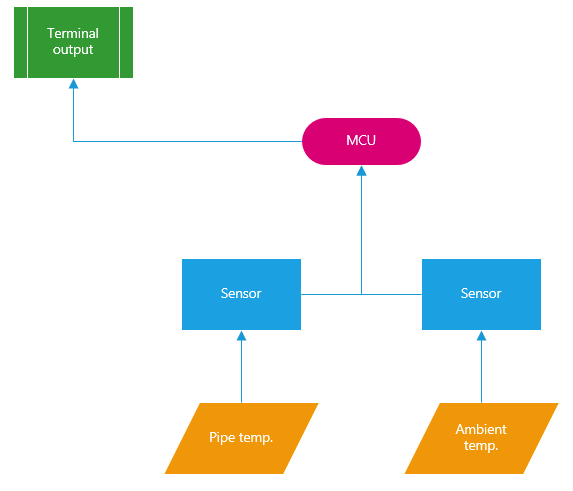
\includegraphics[width=0.5\textwidth]{figures/Phase1.PNG}
\end{figure}








